\documentclass[11pt]{beamer}
%\usetheme{Pittsburgh}
\usepackage[utf8]{inputenc}
\usepackage[german]{babel}
\usepackage{amsmath}
\usepackage{amsfonts}
\usepackage{tikz}
\usetikzlibrary{arrows,positioning,shapes,patterns}
\usepackage{amssymb}
\author{Jonas Ackermann and Lasse Schuirmann}
\title{Discrete Inverse Problems - Solving Real Problems}
%\setbeamercovered{transparent} 
%\setbeamertemplate{navigation symbols}{} 
%\logo{} 
%\institute{} 
\date{19.09.2014} 
%\subject{}
%\setcounter{tocdepth}{1}
\begin{document}
% Styles for diagram
\tikzstyle{decision} = [diamond, draw, 
    text width=4.5em, text badly centered, node distance=3cm, inner sep=0pt]
\tikzstyle{block} = [rectangle, draw, 
    text width=5em, text centered, rounded corners, minimum height=4em]
\tikzstyle{line} = [draw, -latex']
\tikzstyle{cloud} = [draw, ellipse, node distance=3cm,
    minimum height=2em]

\begin{frame}
\titlepage
\end{frame}


\begin{frame}
\tableofcontents
\end{frame}


\section{Barcode Reader}
\begin{frame}{Barcode Reader}
\begin{center}

\includegraphics[scale=0.5]{Barcode_example.PNG} 
\end{center}
\end{frame}


\begin{frame}{Barcode Reader}
\begin{center}
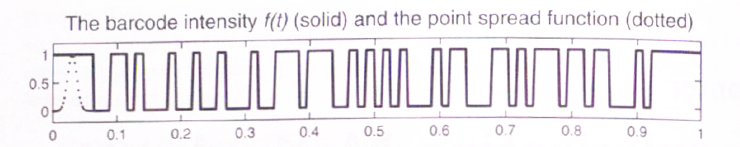
\includegraphics[scale=0.5]{Barcode_f.PNG} 
\end{center}
\end{frame}


\subsection{Modellierung}
\begin{frame}{Modellierung des Barcode Readers (1)}
\begin{center}
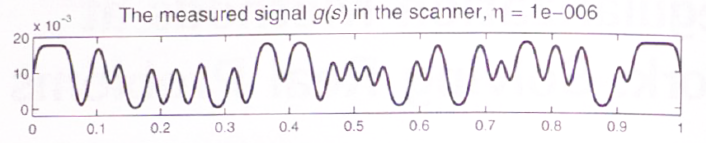
\includegraphics[scale=0.5]{Barcode_g.PNG} 
\end{center}
\end{frame}


\begin{frame}{Modellierung des Barcode Readers (2)}
\[g(s) = \int\limits_{0}^1 f(t) \cdot h(s-t) dt = \int\limits_{0}^1 f(t) \cdot e^{-\left(s-t \over \varsigma\right)^2} dt, \, \, \, \, \, \, 0 \leq s \leq 1 \]
\end{frame}


\begin{frame}{Barcode Reader: Faltung}
\[
g(s) = \int\limits_{0}^1 f(t) \cdot h(s-t) dt
\]

Entspricht einer Faltung $\rightarrow$ Invers: Dekonvolution (Entfaltung)
\end{frame}


\begin{frame}{Barcode Reader: Diskretisierung}
\[
a_{ij} = K(s_i, t_j) = \frac{1}{n} e^{-\left(i-j \over \varsigma n\right)^2}, \,\,\,\,\, i,j = 1, ..., n
\]

\[\]

\[
\mbox{Mit: } s_i = \frac{(i- \frac{1}{2})}{n}, \,\,\,\, t_j = \frac{(j - \frac{1}{2})}{n}
\]
\end{frame}


\subsection{Rekonstruktion}
\begin{frame}{Barcode Reader: Rekonstruktion}
\begin{center}
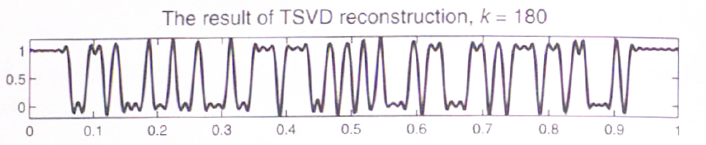
\includegraphics[scale=0.5]{Barcode_TSVD.PNG} 
\end{center}
\end{frame}


\section{Data Model Mismatch}
\begin{frame}{Data Model Mismatch (1)}

Modell basiert auf Annahmen über Daten. Annahmen erfüllt?

\end{frame}



\begin{frame}{Data Model Mismatch (2)}

\begin{center}

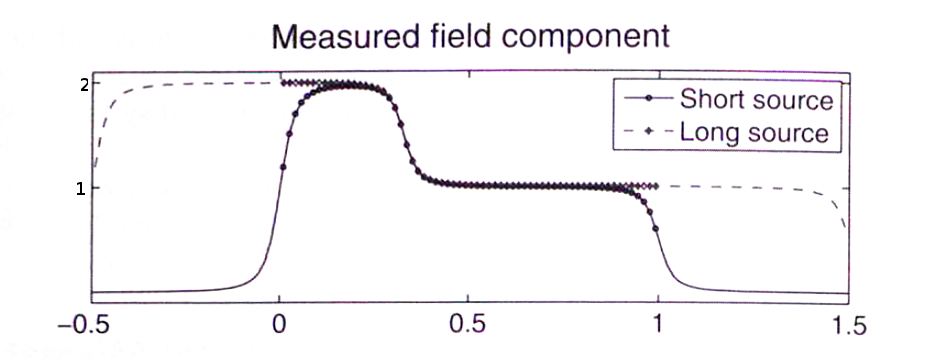
\includegraphics[scale=0.5]{DataModel_graph.PNG} 

\end{center}

\end{frame}


\section{Inverse Crime}
\begin{frame}{Inverse Crime (1)}
\begin{center}
\begin{tikzpicture}[
    pre/.style={=stealth',semithick},
    post/.style={->,shorten >=1pt,>=stealth',semithick}
    ]

\node[draw] (origin) {$f(t)$};

\node[right=of origin](dummy){};

\node[draw, below=of dummy](Inverse){Inverses Modell};
\node[draw, above=of dummy](Modell){Modell};   
\node[draw,right=of dummy](blurred){$g(s)$};

 \draw[post,rounded corners=5pt] (Modell)-|(blurred)  ;   
 \draw[post,rounded corners=5pt] (blurred)|-(Inverse)  ;   
 \draw[post,rounded corners=5pt] (origin) |- (Modell);
  \draw[post,rounded corners=5pt] (Inverse) -| (origin);

\end{tikzpicture}
\end{center}



Kann das Modell anhand des Modells selbst geprüft werden?
\end{frame}



\begin{frame}{Inverse Crime (2)}

\begin{center}

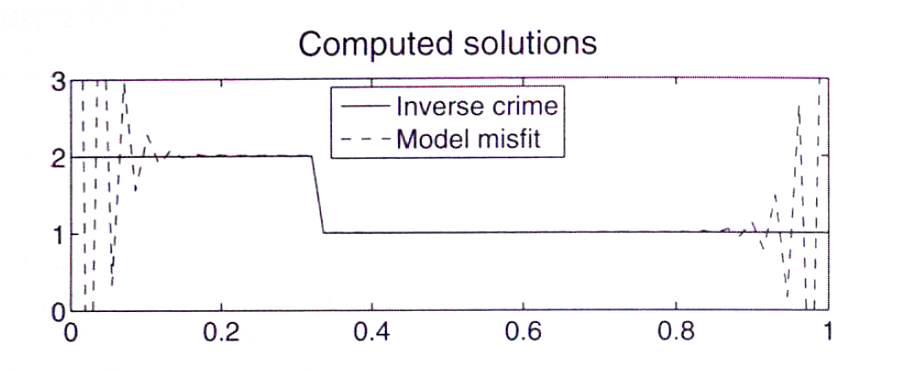
\includegraphics[scale=0.5]{InverseCrime} 

\end{center}

\end{frame}


\section{Grenzbedingungen}
\begin{frame}{Grenzbedingungen (1)}
Was passiert ausserhalb der Grenzen im Originalsignal?

Wie wird das gegebene Signal dadurch beeinflusst?
\end{frame}


\subsection{Mögliche Ansätze}
\begin{frame}{Grenzbedingungen (2)}
Häufig sind Annahmen nötig:
\begin{itemize}
\item Originalfunktion null ausserhalb der Grenzen?
\item Originalfunktion verhält sich ähnlich wie innerhalb?

$\rightarrow$ Reflektierende Grenzbedingung.
\end{itemize}
\end{frame}


\subsection{Reflektierende Grenzbedingung}
\begin{frame}{Reflektierende Grenzbedingung (1)}
\[
f_{BC}(t) = \begin{cases}
f(-t), & -1 < t < 0,\\
f(t),  & 0 \leq t \leq 1,\\
f(2-t),& 1 < t < 2.\\
\end{cases}
\]
\end{frame}


\begin{frame}{Reflektierende Grenzbedingung (2)}
\begin{align}
g_{BC}(s) & = \int\limits_{-1}^2 K(s,  t) f_{BC}(t) dt \notag \\
          & = \int\limits_{-1}^0 K(s,  t) f_{BC}(t) dt
            + \int\limits_{ 0}^1 K(s,  t) f_{BC}(t) dt
            + \int\limits_{ 1}^2 K(s,  t) f_{BC}(t) dt \notag \\
          & = \int\limits_{ 0}^1 K(s, -t) f     (t) dt
            + \int\limits_{ 0}^1 K(s,  t) f     (t) dt
            + \int\limits_{0 }^1 K(s,2-t) f     (t) dt \notag
\end{align}
\end{frame}


\begin{frame}{Reflektierende Grenzbedingung (3)}
 \[K_{BC} = K(s, -t) + K(s,  t) + K(s, 2-t)\]
\end{frame}


\begin{frame}{Reflektierende Grenzbedingung (4)}
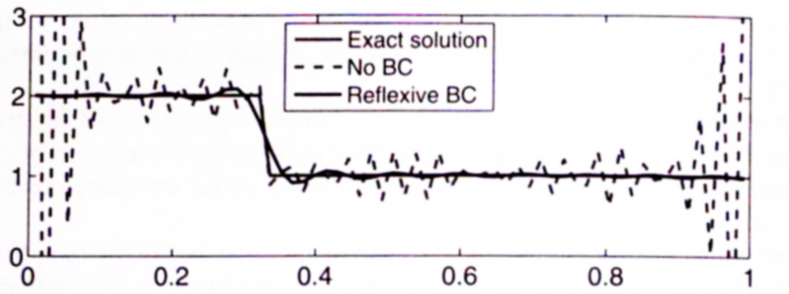
\includegraphics[scale=0.38]{boundary_conditions} 
\end{frame}


\section{Diskretisierung}
\begin{frame}{Matrix}
Zurück zum Diskreten!
\end{frame}


\begin{frame}{Toeplitz und Zyklische Matrizen}
\[
\begin{pmatrix}
{\color{red}    1} & {\color{blue}   2} & {\color{green}  4} &                6 \\
{\color{yellow} 0} & {\color{red}    1} & {\color{blue}   2} & {\color{green} 4}\\
{\color{cyan}   3} & {\color{yellow} 0} & {\color{red}    1} & {\color{blue}  2}\\
                5  & {\color{cyan}   3} & {\color{yellow} 0} & {\color{red}   1}\\
\end{pmatrix}
\,\,\,\,\,\,\,\,\,
\begin{pmatrix}
{\color{red}    1} & {\color{blue}   2} & {\color{green}  4} & {\color{yellow} 0}\\
{\color{yellow} 0} & {\color{red}    1} & {\color{blue}   2} & {\color{green}  4}\\
{\color{green}  4} & {\color{yellow} 0} & {\color{red}    1} & {\color{blue}   2}\\
{\color{blue}   2} & {\color{green}  4} & {\color{yellow} 0} & {\color{red}    1}\\
\end{pmatrix}
\]
\end{frame}


\begin{frame}{A ist eine Toeplitz Matrix}
\[
h[i-j] := a_{ij} (= K(s_i, t_j))
\]
\[
(x \star h)[i] = \sum\limits_{j=0}^{N-1} x[j] \cdot h[i-j] = b[i]
\]
\[
\begin{array}{c|cccc}
b[i]/x[j] & x[0] & x[1] & ... & x[N-1]  \\
\hline
b[0]     & h[0] & h[-1] & \cdots & h[-N+1] \\
b[1]     & h[1] & h[0] & \cdots & h[-N+2]  \\
\vdots  & \vdots & \vdots & \ddots & \vdots \\
b[N-1] & h[N-1] & h[N-2] & \cdots & h[0]  \\
\end{array}
\]
\end{frame}


\begin{frame}{Matrix: Berücksichtigung von Grenzbedingungen (1)}
Korrekturterme notwendig.

Reflektierende Grenzbedingungen - Erinnerung:

\[K_{BC} = K(s, -t) + K(s,  t) + K(s, 2-t)\]

Also: was fehlt in der Matrix?
\pause

$A^l$ und $A^r$!
\end{frame}


\begin{frame}{Matrix: Berücksichtigung von Grenzbedingungen (2)}
Beispielhaft für $A^l$:
\[
a^l_{ij} = K(s_i, -t_j) = \frac{1}{n} e^{-\left(i+j-1 \over \varsigma n\right)^2}, \,\,\,\,\, i,j = 1, ..., n
\]

Daraus ergibt sich $A_{BC}$:

\begin{center}
$A_{BC} = A + A^l + A^r$ 
\end{center}
\end{frame}


\section{Zweidimensionale Faltung}
\begin{frame}{Zweidimensionale Faltung - Ein Beispiel}
\begin{center}
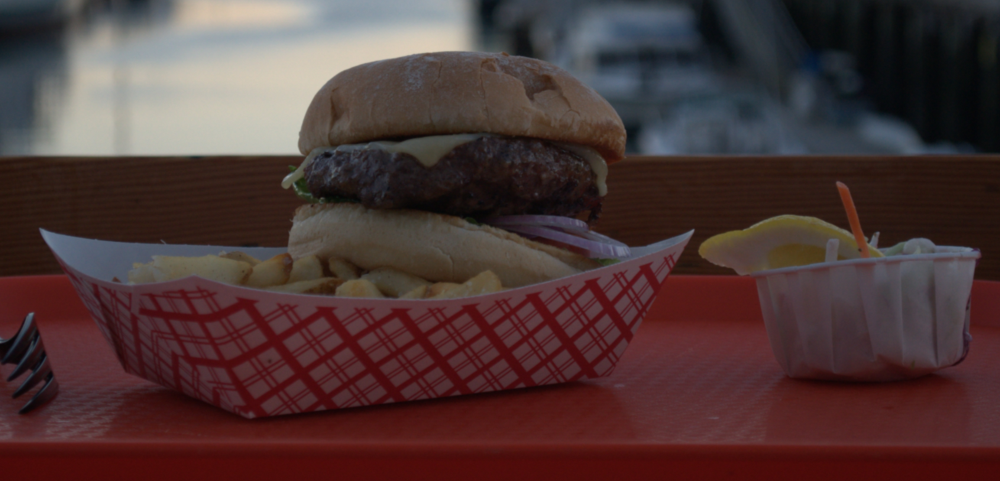
\includegraphics[scale=1]{Burger_unblurred} 


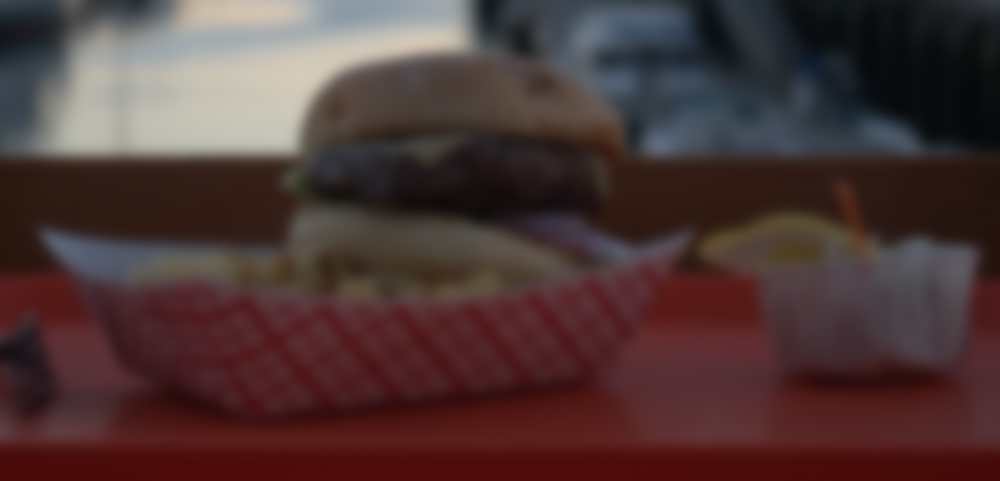
\includegraphics[scale=1]{Burger_blurred} 
\end{center}
\end{frame}


\begin{frame}{Zweidimensionale Faltung - Theorie}
\[
\int\limits_0^1
  \int\limits_0^1
    K(\textbf{s},\textbf{t}) \cdot f(\textbf{t}) dt_1 dt_2
= g(\textbf{s})
\,\,\,\,\,\,
s \in [0,1] \times [0,1].
\]

Mit $\textbf{s} = (s_1,s_2)$ und $\textbf{t} = (t_1,t_2)$
\end{frame}

\begin{frame}{Umsetzung (1)}


Regularisierungs-Methode?

$\newline$

Parameter-Wahl-Methode?

$\newline$

Implementierung?

\end{frame}

\begin{frame}{Umsetzung (2)}

Performanz $\rightarrow$ Ausnutzbare Matrixeigenschaften?

$\newline$

Realitätsnähe $\rightarrow$ Womit Algorithmus testen?

\end{frame}

\section{Fazit}
\begin{frame}{Fazit}
\begin{itemize}
\item Benötigte Grundlagen:
\pause
  \begin{itemize}
  \item Toepliz Matrizen
  \pause
  \item Zirkuläre Matrizen
  \pause
  \item Regularisierung
  \pause
  \item Faltung, natürlich!
  \pause
  \end{itemize}
\item Beispiele für diskrete inverse Probleme:
\pause
  \begin{itemize}
  \item Barcode Reader
  \pause
  \item Bildunschärfe
  \pause
  \end{itemize}
\item Dinge die es zu beachten gibt:
\pause
  \begin{itemize}
  \item Grenzbedingungen
  \pause
  \end{itemize}
\item Validierung von Problemlösungen:
\pause
  \begin{itemize}
  \item Inverse Crime
  \pause
  \item Data/Model Mismatch
  \end{itemize}
\end{itemize}
\end{frame}


\end{document}
